%-------------------------------------------------------------
\subsection{Example 2} \label{sec:ch5:example2}

%-------------------------------------------------------------
\subsubsection{Description}
For the second example, we will consider the problem on pp.~120--122 from Ref.~\cite{Bryson1975a} and in Ref.~\cite{Bryson1963a}:
\begin{subequations}%%
\begin{align}
\min_{u} \quad & \frac{1}{2}\int_{0}^{1} u^2 dt \\
\text{subject to:} \quad  & \dot{\bm{\xi}} = \begin{bmatrix} \xi_2 \\ u \end{bmatrix} \\
& \xi_1(0) = 0, \quad \xi_1(1) = 0, \quad \xi_2(0) = 1, \quad \xi_2(1) = -1 \\
& \xi_1(t) \leq 1/9
\end{align}
\end{subequations}%

\noindent This problem is similar to \nameref{sec:ch5:example1} but, now has a path constraint.
The structure-based problem description for this example is:%
\allowdisplaybreaks[1]
\begin{subequations}%
\begin{gather}
% Lagrange term
\mathcal{L}\xind{1}.\xvar{left} = 1, \quad \mathcal{L}\xind{1}.\xvar{right} = 1, \quad \mathcal{L}\xind{1}.\xvar{matrix} = 1/2 \\
% system dynamics
\bm{A} = \begin{bmatrix} 0 & 1 \\ 0 & 0
\end{bmatrix}, \quad \bm{B} = \begin{bmatrix} 0 \\ 1
\end{bmatrix} \\
% linear equality constraints
\mathcal{LB}\xind{1}.\xvar{right} = 4, \quad \mathcal{LB}\xind{1}.\xvar{matrix} = \begin{bmatrix} 0 & 1 \end{bmatrix}\tran \\
\mathcal{LB}\xind{2}.\xvar{right} = 5, \quad \mathcal{LB}\xind{2}.\xvar{matrix} = \begin{bmatrix} 0 & -1 \end{bmatrix}\tran \\
\mathcal{UB}\xind{1}.\xvar{right} = 4, \quad \mathcal{UB}\xind{1}.\xvar{matrix} = \begin{bmatrix} 0 & 1 \end{bmatrix}\tran \\
\mathcal{UB}\xind{2}.\xvar{right} = 5, \quad \mathcal{UB}\xind{2}.\xvar{matrix} = \begin{bmatrix} 0 & -1 \end{bmatrix}\tran \\
\mathcal{UB}\xind{3}.\xvar{right} = 2, \quad \mathcal{UB}\xind{3}.\xvar{matrix} = \begin{bmatrix}\ell & \infty \end{bmatrix}\tran % \\
\end{gather}
\end{subequations}%%
\allowdisplaybreaks[0]%

\noindent The \textsc{Matlab} code is in Sec.~\ref{sec:ex2-code}.

%-------------------------------------------------------------
\subsubsection{Solution}

\begin{figure}
\centering

\begin{subfigure}{0.5\textwidth}
\centering
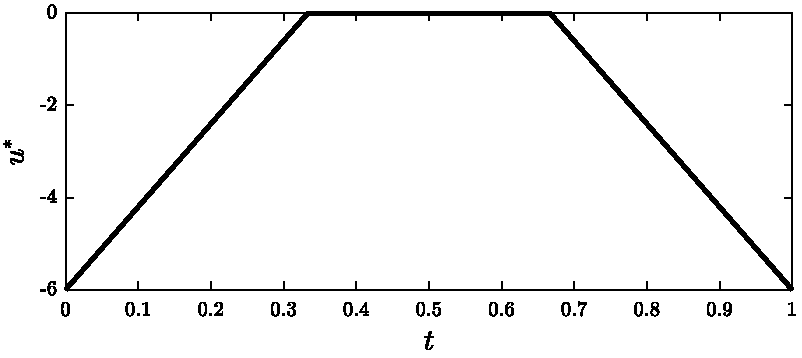
\includegraphics[width=\textwidth]{../ch5/figures/ex2sol-controls}%
\caption{Control.}
\label{fig:ch5:ex2sol:controls}
\end{subfigure}%
\begin{subfigure}{0.5\textwidth}
\centering
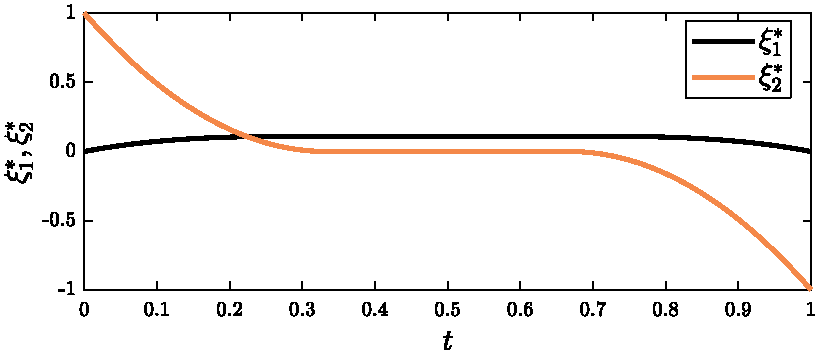
\includegraphics[width=\textwidth]{../ch5/figures/ex2sol-states}%
\caption{States.}
\label{fig:ch5:ex2sol:states}
\end{subfigure}%

\caption{Solution for \nameref{sec:ch5:example2}.}
\label{fig:ch5:ex2sol}
\end{figure}

It can be shown that the control trajectory that minimizes the objective while satisfying the constraints when $0 < \ell \leq 1/6$ is:
\begin{align}
u^*(t) = \begin{cases}
-\frac{2}{3\ell}\left( 1 - \frac{t}{3\ell} \right) & 0 \leq t < 3\ell \\
0 & 3\ell \leq t < 1 - 3\ell \\
-\frac{2}{3\ell}\left( 1 - \frac{1-t}{3\ell} \right) & 0 \leq t \leq 3\ell \\
\end{cases}
\end{align}

\noindent with an optimal objective function value of:
\begin{align}
\Psi^* = \frac{4}{9\ell}
\end{align}

\noindent A problem parameter value of $\ell = 1/9$ will be used, and with this value, $\Psi^* = 4$.
The optimal trajectories for both the control and states are shown in Fig.~\ref{fig:ch5:ex2sol}.

%-------------------------------------------------------------
\subsubsection{Numerical Results}

The convergence results for the eight tested schemes are shown in Fig.~\ref{fig:ch5:ex2sens}.
All schemes, including the PS-based schemes, achieve similar sublinear convergence rates, and this is due to the path constraint.
For the ED meshes, if $N_t-1$ was a multiple of 3, then nodes values of $1/3$ and $2/3$ would be directly included in the mesh.
Otherwise, the locations where the path constraint changes activity (in the true solution) would not be included.
Therefore, there is slow convergence due to errors around these points.
However, when $N_t=4$ with ED-HS-CQHS (5) or ED-RK4-CQHS (6), all relevant quantities (states, control, and objective value) are accurate within the machine precision!
Such accuracy with a minimal number of node points was previously only possible with specifically constructed multiple-interval PS methods \cite{Herber2015a}.
Since the optimal control policy is piecewise linear, the CQHS method is exactly accurate for $u^2$ terms.
Furthermore, the states are piecewise quadratic and cubic and both the HS and RK4 methods exactly approximate these dynamics.
Therefore, schemes (5,6) exactly represent the original problem.

% new paragraph
Ignoring the favorable meshes and looking at the local worst errors, we still see (5,6) performing the best along with ED-ZOH-CEF (1) (except with respect to the controls).
These are followed closely by the other methods except for ED-EF-CEF (2), which was the worst method again.
These results for the PS-based schemes demonstrate the potentially issue with using a single global polynomial when path constraints are present \cite{Darby2009a, Darby2011a}.
Multiple-interval PS methods would be more suitable for this type of problem (see Sec.~\ref{sec:ch5:multipleinterval}).

\begin{figure}%
\centering

{\footnotesize Local maximum values (local minimum values are in a thinner, translucent color):}


\includegraphics[width=\textwidth]{../ch5/figures/ex1_sens_legend}%

\vspace{1mm}

\begin{subfigure}{0.5\textwidth}
\centering
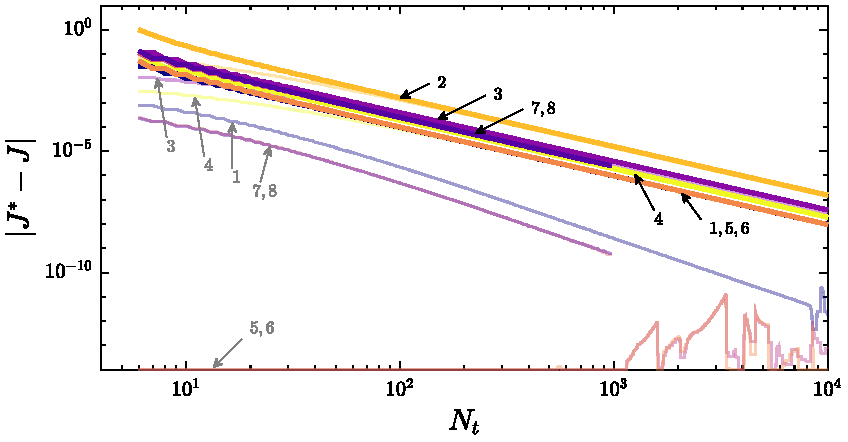
\includegraphics[width=\textwidth]{../ch5/figures/ex2_sens_objective}%
\caption{Objective error.}
\label{fig:ch5:ex2sens:objective}
\end{subfigure}%
\begin{subfigure}{0.5\textwidth}
\centering
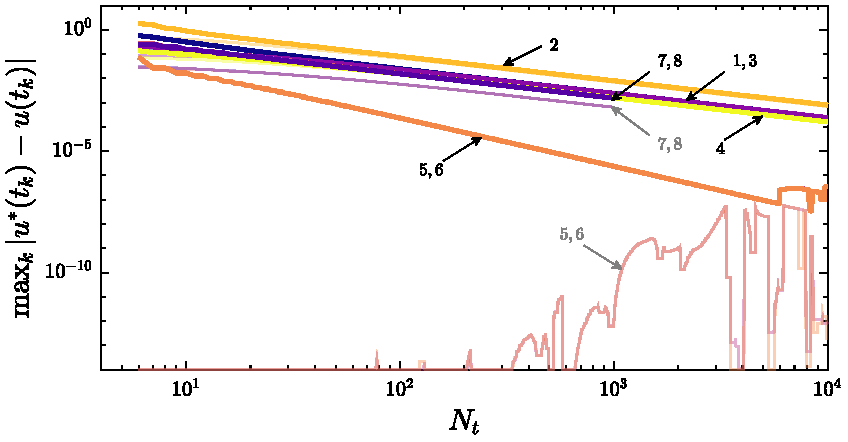
\includegraphics[width=\textwidth]{../ch5/figures/ex2_sens_control}%
\caption{Control error.}
\label{fig:ch5:ex2sens:control}
\end{subfigure}%

\begin{subfigure}{0.5\textwidth}
\centering
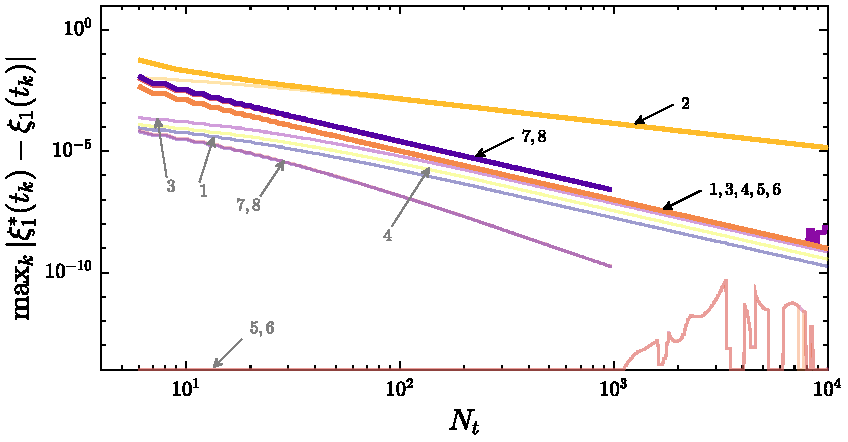
\includegraphics[width=\textwidth]{../ch5/figures/ex2_sens_state_1}%
\caption{$\xi_1$ error.}
\label{fig:ch5:ex2sens:state:1}
\end{subfigure}%
\begin{subfigure}{0.5\textwidth}
\centering
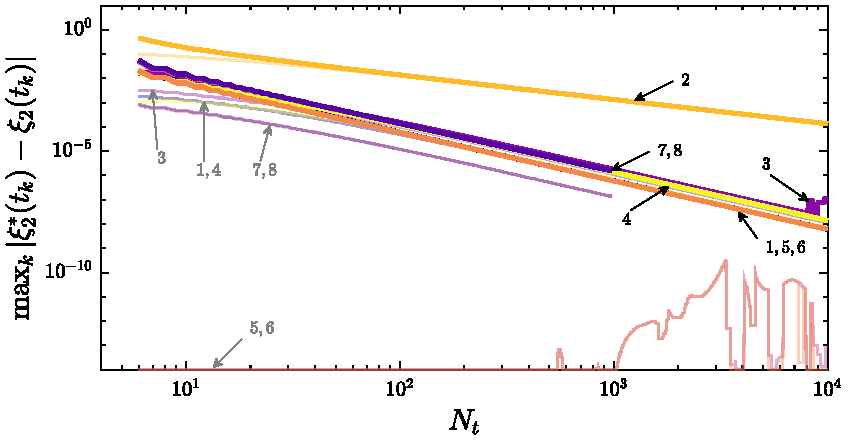
\includegraphics[width=\textwidth]{../ch5/figures/ex2_sens_state_2}%
\caption{$\xi_2$ error.}
\label{fig:ch5:ex2sens:state:2}
\end{subfigure}%

\caption{Numerical results for \nameref{sec:ch5:example2}.}
\label{fig:ch5:ex2sens}
\end{figure}